\section{Field Programmable Gate Array}

\subsection{An Overview of FPGA}
Field Programmable Gate Array (FPGA) is a type of integrated circuit (IC)
containing a matrix of logic cells that can be programmed by a user to act
as an arbitrary integrated circuit.

The first field programmable gate array is manufactured by Xilinx
in 1985. However, compared with the widespread of computers, FPGA
was primarily made use of in telecommunications and networking in
the 1990s due to both the sophistication and the volume of the production.

Using the pre-built logic blocks and
programmable routing resources, you can configure these chips to implement
custom hardware functionality in high performance. For example, one can implement a
interrupt controller, a digital filter or even a processor on the basic of
FPGA.

In the past, FPGA technology could be used only by
engineers with a deep understanding of digital hardware design. Thus FPGA is
not as widely use as general purpose processor around the world. But in
the recent years, some companies encapsulated the underlining details of
FPGA and rised several suits of development tools kits to provide a higher
abstract interface for develops. The developers who designing the FPGA now
just need to task in the software and compile them down to a configuration
file or bitstream that contains information on how to components should be
wired together, which makes the task much easier and more and more
developers devotes their energies to FPGA.

\subsection{The Architecture of FPGA}

A typical layout of FPGA (see Figure~\ref{fig:fpga_arch}) is an array of
interconnected programmable logic blocks or configurable logic blocks. It
provides the designer with programmable logic blocks that contain the pool
of combinatorial blocks and flip-flops to be used in the design. Logic is
often used in conjunction with memory. Clock conditioning has also become
commonplace, and support in the form of Delay Locked Loops (DLLs). Phase
Locked Loops (PLLs) is also provided inside the same silicon chip. Finally,
an FPGA chip does not lead a solitary life isolated from the rest of the
world. It needs to be easily interfaced to other chips or external signals.
In order to make this interfacing easier, FPGA vendors have invested a
great deal of effort in enhancing the flexibility of the input/output
blocks behind the chip pads. Each pad can serve as an input, an output, or
both. The list of electrical standards supported is extensive, and novel
techniques for maximizing bandwidth, such as clocking data in using both
edges of the clock, are widely supported~\cite{fpgaintro}.

\begin{figure}
  \centering
  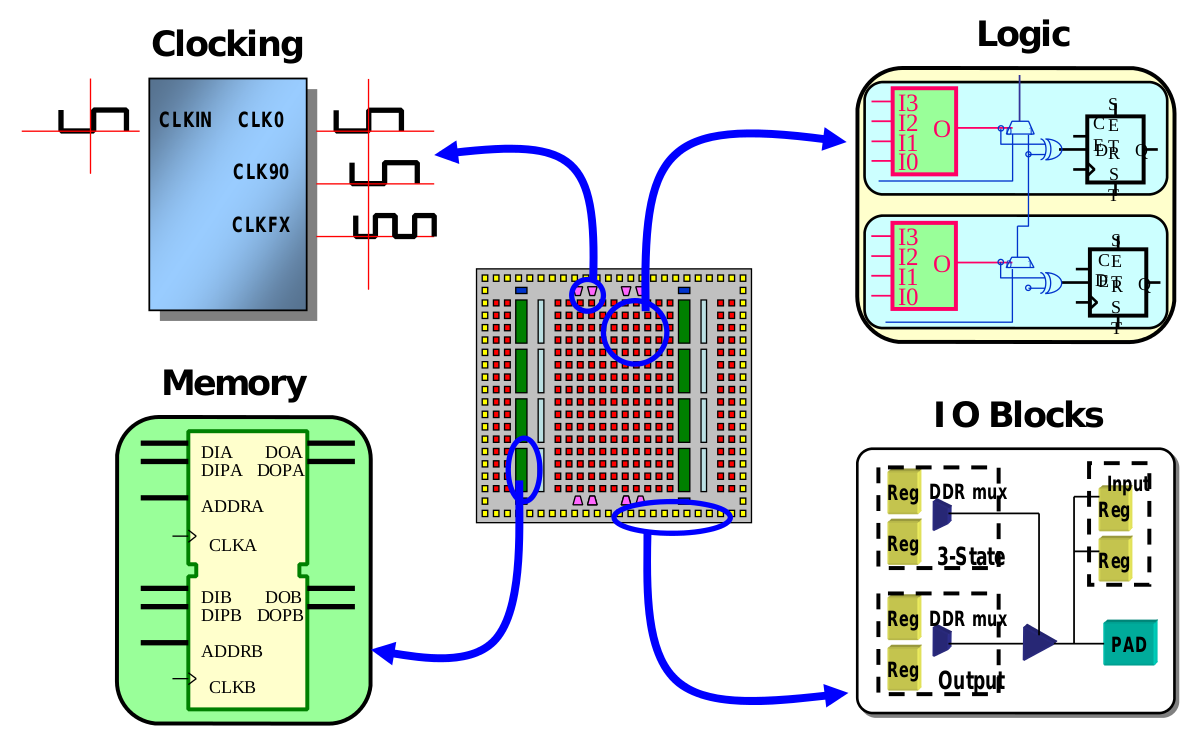
\includegraphics[scale=0.25]{img/fpga_arch.png}
  \caption{Typical structure of modern FPGA}
  \label{fig:fpga_arch}
\end{figure}

Xilinx is the largest vendors of modern FPGA , their latest product, such
as Spartan-3 generation, general consist of five fundamental programmable
functional elements, configurable Logic Blocks (CLBs), Input/Output Blocks
(IOBs), BLOCK RAM, Multiplier Blocks, and Digital Clock Manager (DCM).

\begin{itemize}

  \item \emph{Configurable Logic Blocks (CLBs)} contain flexible Look-Up
    Tables (LUTs) that implement logic plus storage elements used as
    flip-flops or latches. CLBs perform a wide variety of logical functions
    as well as store data.

  \item \emph{Input/Output Blocks (IOBs)} control the flow of data between
    the I/O
    pins and the internal logic of the device. IOBs support bidirectional
    data flow plus 3-state operation. Supports a variety of signal
    standards, including several high-performance differential standards.
    Double Data-Rate (DDR) registers are included.

  \item \emph{Block RAM} provides data storage in the form of 18-Kbit
    dual-port
    blocks.

  \item \emph{Multiplier Blocks} accept two 18-bit binary numbers as inputs
    and
    calculate the product. The Spartan-3A DSP platform includes special DSP
    multiply-accumulate blocks.

  \item \emph{Digital Clock Manager (DCM)} Blocks provide self-calibrating,
    fully
    digital solutions for distributing, delaying, multiplying, dividing,
    and phase-shifting clock signals.
\end{itemize}

These elements are organized as shown in Figure~\ref{fig:spartan_arch},
using the Spartan-3A FPGA
array as an example. A dual ring of staggered IOBs surrounds a regular
array of CLBs in the Spartan-3 and Extended Spartan-3A family. The
Spartan-3E family has a single ring of inline IOBs. Each block RAM column
consists of several 18-Kbit RAM blocks. Each block RAM is associated with a
dedicated multiplier. The DCMs are positioned with two at the top and two
at the bottom of the device, plus additional DCMs on the sides for the
larger devices.

\begin{figure}[h]
  \centering
  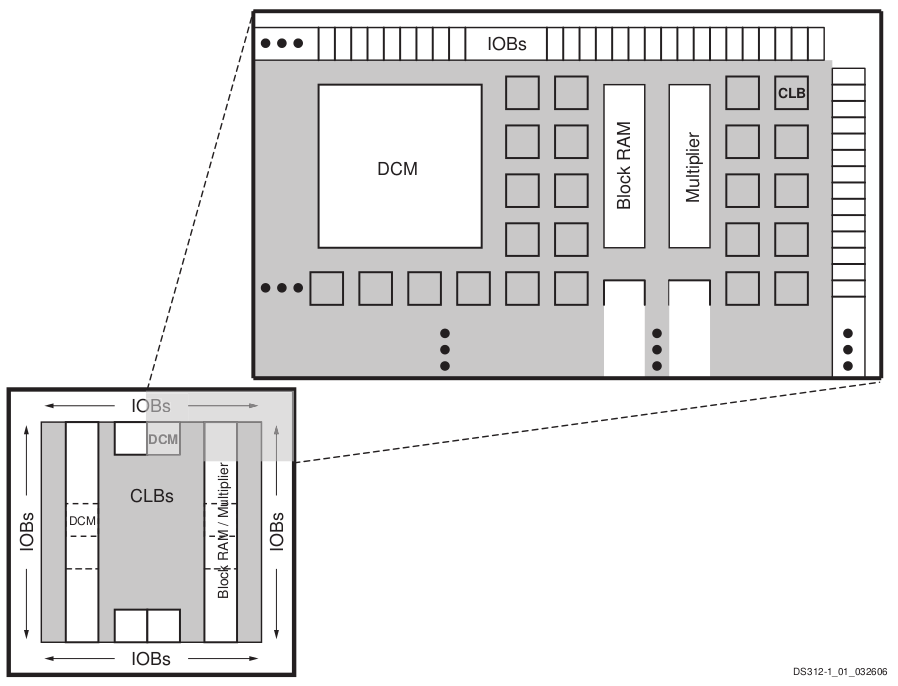
\includegraphics[scale=0.3]{img/spartan_arch.png}
  \caption{Spartan-3A Platform Architecture}
  \label{fig:spartan_arch}
\end{figure}

The Spartan-3 generation features a rich network of traces that
interconnect all five functional elements, transmitting signals among them.
Each functional element has an associated switch matrix that permits
multiple connections to the routing\cite{fpgaug}.

\subsection{Designing FPGA with Maxcompiler}

The usual way to design FPGAs is to write a behavioral model in
a Hardware Description Language (HDL), like Verilog or VHDL, which
supports concurrency and synchronous circuits. Concurrency allows
you to create fully parallel, independent processes, each describing
how to update some variables continuously. Synchronous circuits, instead,
are those made of flip-flops that change their state only on the edge
of some clock signal.

After the design has been written and verified with an HDL simulator,
a compiler creates a list of all the logic gates and the wires (nets)
that must connect them to reproduce the functionality of the HDL model.
After this logic synthesis, layout programs read the netlist and several
constraints files to find out which logic gates inside the FPGAs must
be used and which physical, internal wires must connect them to each
other. The end result is the bit file that the FPGA reads at power-up.

The above kind of FPGA configuring developing is still an obstruct for
those who seldom care much about hardware or digital circuit. In order to
make full use of FPGA, Maxeler Inc, develops a compiler where software
engineer can perform configuring developing with their daily used
developing language, such as C, and Java.

\subsubsection{Maxeler Acceleration Technology}

\emph{Maxcompiler} is a commercial product that is manufactured by Maxeler.
It is a compiler system for Maxeler hardware acceleration solutions using
FPGAs. The compiler system is a good assistant for software engineering
developer to create FPGA configuring because it has a higher abstract of
the underlining subtle hardware information, and then provide a set of
Application Interface for developers.

Figure~\ref{fig:maxeler_acceleration_system} have a sketch of Maxeler
acceleration system architecture. The system comprises several FPGAs
attached directly to the local memory and to a host CPU via PCI Express.

\begin{figure}
  \centering
  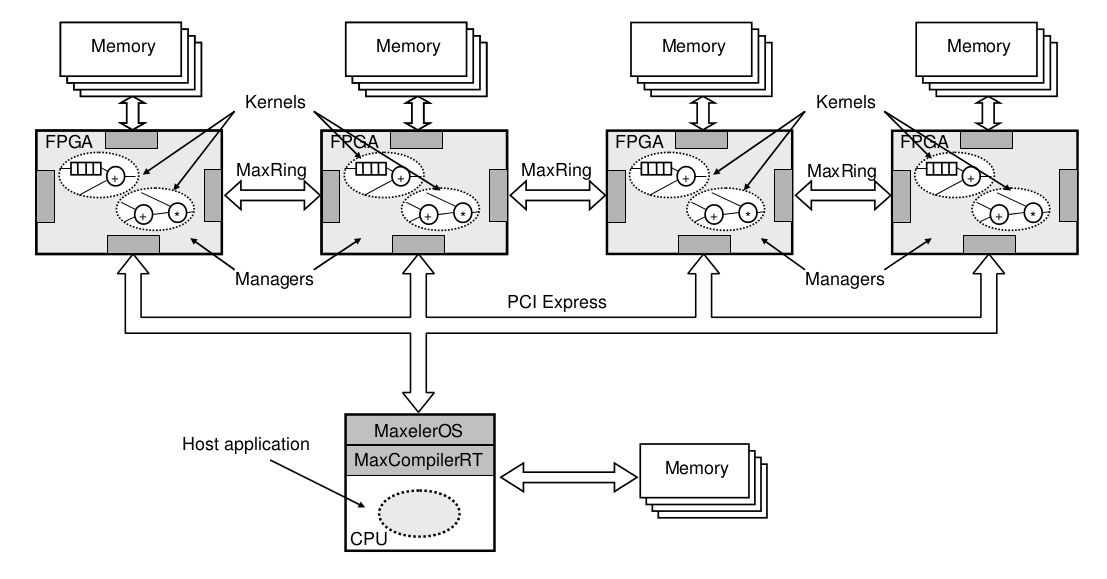
\includegraphics[scale=0.35]{img/overview_of_maxeler_acceleration_system.png}
  \caption{An overview of Maxeler acceleration system}
  \label{fig:maxeler_acceleration_system}
\end{figure}

While developing the application, develops identify the runtime intensive part
and tunning them into FPGA configuration, which is called \emph{kernel} and
\emph{manager} in the acceleration system. After all the configured FPGA
files are compiled and downloaded into FPGA EEPROM, the host (CPU) code
communicate with FPGA with the help of \emph{Maxeler OS}. The Maxeler OS
provide a set of API called \emph{MaxCompierRT}, a runtime library to load
the configuration to FPGA and transfer data from/to FPGA.

The programming paradigm of FPGA designing is different from the general
programming paradigm, such as C/C++. The FPGA gains it high efficiency from
the parallel working of the different Configurable Logic Block (CLB). The
program describes the computations structurally (in space) rather than
specifying the sequence of processor instructions (in
time)\cite{max_white_paper}.

\subsubsection{Development Flow}
If the developer want to accelerate an application after he identifies the
runtime intensive part of the program, what he needs includes three parts,
designing the kernel, manager configuration and adapt the host application.
All the three parts can be easily implemented with the help of Maxeler
compiler tools. Figure \ref{fig:development_flow} presents the development flow with the main
components of MaxCompiler.

\begin{figure}[h]
  \centering
  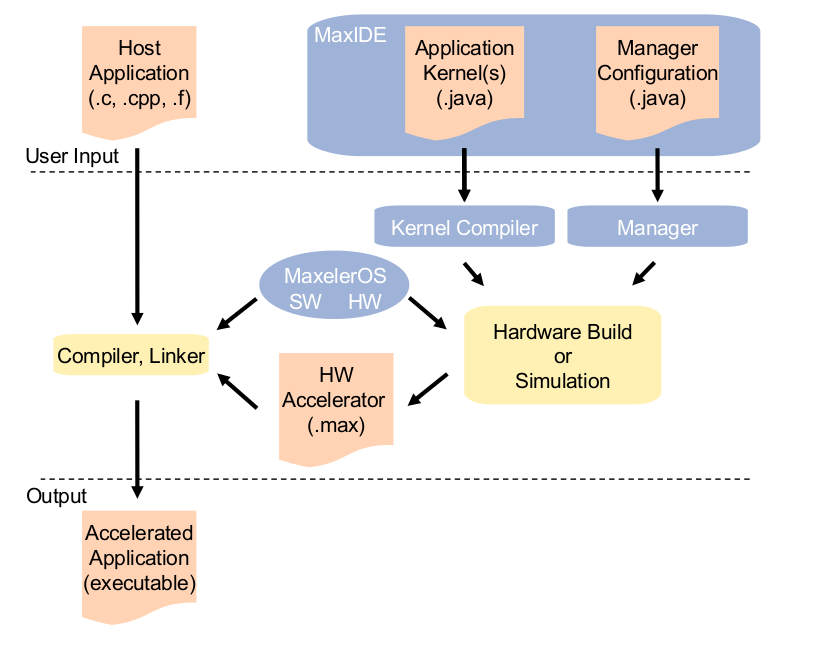
\includegraphics[scale=0.4]{img/development_flow.png}
  \caption{Maxeler development flow}
  \label{fig:development_flow}
\end{figure}

The first stage, designing the kernel, is the most critical part of the
acceleration. Kernel has the similar meaning with that in CUDA GPU
programming, which refers to the most computationally-demanding part that
should be executed in the FPGA/GPU board. Java, the well-known high level
language is used to develop the kernel. Here we just the syntax of Java,
excluding the massive Java library. In addition, the Maxeler provides a set
of library that use to configure the kernel with the help of the
MaxCompiler. Instead of using the phase ``programming to configure kernel
with Java'', it is more appropriate to say ``designing the configure kernel
with Java'', because paradigm of designing the FPGA application with
MaxCompiler is to describe the structure of the logic, rather than telling
the FPGA the sequence of the process instructions, which we use in the
general purpose programming.

When the kernel is well configured, we need to set up a manager for it. The
manager is responsible for how to set up the kernel, for example, pass the
parameter to kernel that kernel expects. What's more, the manager is also
responsible to cooperate the kernels together if there are multiple
kernels, or multiple FPGA boards working for the same problem. The manager
can configure the kernel for simulation or for real work kernel.
Configuring the kernel for simulation is preferred because it saves time to
generate it. A full hardware build may take you hours or even weeks
depending on the complexity of the kernel.

Whenever the simulation kernel or the hardware kernel is build, it is
possible to linked it with the host application. Maxeler provides a set of
runtime library in C/C++ and Fortran to help the programmer to develop. The
communication between the local machine and FPGA device is via the runtime
library and interface, which could help the developer to transform data
from/to the FPGA Device.

The MaxCompiler can link them together in the last stage of the compilation
and generate the ordinary binary executable file.

\subsection{Advantage of FPGA Designing}

FPGA chip adoption across all industries is driven by the fact that FPGAs
combine the best parts of ASICs and processor-based systems. FPGAs provide
hardware-timed speed and reliability, but they do not require high volumes
to justify the large upfront expense of custom ASIC design. Reprogrammable
silicon also has the same flexibility of software running on a
processor-based system, but it is not limited by the number of processing
cores available.

Unlike processors, FPGAs are truly parallel in nature, so
different processing operations do not have to compete for the same
resources. Each independent processing task is assigned to a dedicated
section of the chip, and can function autonomously without any influence
from other logic blocks. As a result, the performance of one part of the
application is not affected when you add more processing.

In addition, FPGAs are blurring the lines between hardware and software in systems.
FPGA devices are inherently soft-programmable and may be changed
dynamically during the operation of a system. More compellingly, FPGA devices
now also contain embedded microprocessors within the logic fabric,
and these microprocessors can run Linux. Imagine a Linux computer
with up to millions of gates of flexible logic immediately around
it. One way to grok this new paradigm is to think of the following:
Software is configuration bits for hardware.
